\documentclass[11pt]{scrartcl}
\usepackage[sexy]{evan}
\usepackage{graphicx}
\usepackage{mathtools}
\usepackage{listings}

 %Sets
\newcommand{\N}{\mathbb{N}}
\newcommand{\Z}{\mathbb{Z}}
\newcommand{\F}{\mathbb{F}}
\newcommand{\Q}{\mathbb{Q}}
\newcommand{\R}{\mathbb{R}}
\newcommand{\C}{\mathbb C}
\newcommand{\T}{\mathbb T}
\newcommand{\PP}{\mathbb P}
\newcommand{\supp}{\text{supp }}
\newcommand{\E}{\mathbb E}
\newcommand{\cov}{\operatorname{cov}}
\renewcommand{\Re}{\operatorname{Re}}
\renewcommand{\Im}{\operatorname{Im}}
\newcommand{\<}{\langle}
\renewcommand{\>}{\rangle}



\DeclareMathOperator*{\Var}{Var}
\newcommand{\Hol}{\operatorname{Hol}}

\let \phi \varphi
\let \hat \widehat
\let \mc \mathcal
\let \p \partial
\let \bar \overline
\let \eps \varepsilon
\newcommand\at[2]{\left.#1\right|_{#2}}

%From Topology
\newcommand{\cT}{\mathcal{T}}
\newcommand{\cB}{\mathcal{B}}
\newcommand{\cC}{\mathcal{C}}
\newcommand{\cH}{\mathcal{H}}

%Indicators 
\newcommand{\1}{\textbf{1}} % vector of all 1's
\newcommand{\I}[1]{\mathbb{I}{\left\{#1\right\}}} % indicator function


\usepackage{answers}
\Newassociation{hint}{hintitem}{all-hints}
\renewcommand{\solutionextension}{out}
\renewenvironment{hintitem}[1]{\item[\bfseries #1.]}{}
\declaretheorem[style=thmbluebox,name={Problem}, numberwithin=section]{prob}

\begin{document}
\title{CS 285}
\author{Vishal Raman}
\thispagestyle{empty}
$ $
\vfill
\begin{center}

\centerline{\huge \textbf{CS 285, Lecture Notes}}
\centerline{\Large \textbf{Deep Reinforcement Learning } }
\centerline{Vishal Raman}
\end{center}
\vfill
$ $
\newpage
\thispagestyle{empty}
\tableofcontents
\newpage
%\maketitle

\section{Supervised Learning of Behaviors}
\subsection{Terminology and Notation}
In a normal supervised learning problem, say object recognition, we may have a object $o_t$ that goes through a DNN and the target is a label $a_t$ from a policy $\pi_{\theta}(a_t \vert o_t)$, where $\theta$ represents the parameter of the policy.  The subscripts correspond to a timestep, since we usually assume we are given data in a sequential format.  Unlike usual supervised learning, the action $a_t$ influences $o_{t + 1}$.  This is summarized in the diagram below:
\begin{center}
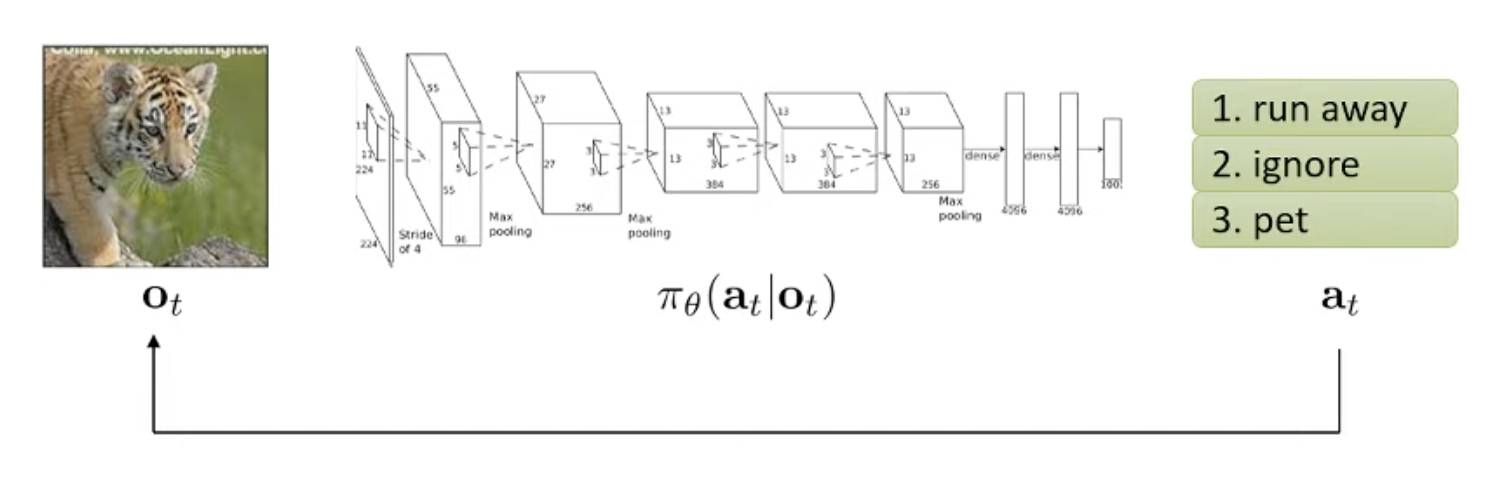
\includegraphics[scale=0.5]{graphics/tiger.png}
\end{center}
Sometimes, we see the policy written as $\pi_{\theta}(a_t \vert s_t)$, where the states $s_t$ are usually assumed to be Markovian while the observations $o_t$ is an observation that results from $s_t$.  

This is illustrated in the graphical model below:
\begin{center}
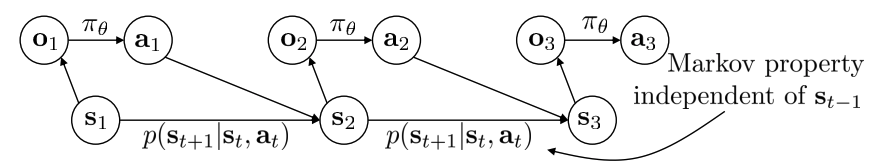
\includegraphics[scale=0.5]{graphics/stateaction.png}
\end{center}

\subsection{Imitation Learning}
We can take an example of self-driving cars.  We start with observations which are images from the car camera and the actions are how we steer the car.  First, we get an image from an expert driving a car and their action.  Then, we record the training data and use supervised learning to map from observations to actions.  This is a type of \textbf{imitation learning} and is sometimes referred to as behavioral cloning, since we are cloning the behavior of the expert driver.  The original deep imitation learning system was proposed in 1989, called ALVINN: Autonomous Land Vehicle In a Neural Network.

We do not expect this to work in theory because if we deviate from the training trajectories(which is essentially inevitable), the expected trajectory will make larger and larger mistakes since they are different from all the training trajectories.  
\begin{center}
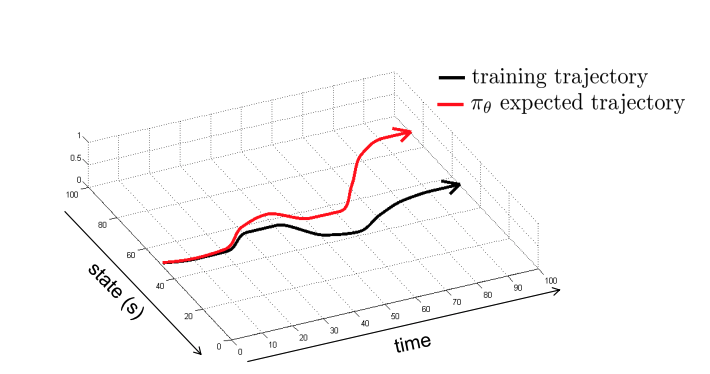
\includegraphics[scale=0.35]{graphics/imitationno.png}
\end{center}

In practice, however, it seems to work well.  Bojarski et al. '16, NVIDIA presented the following algorithm:
\begin{center}
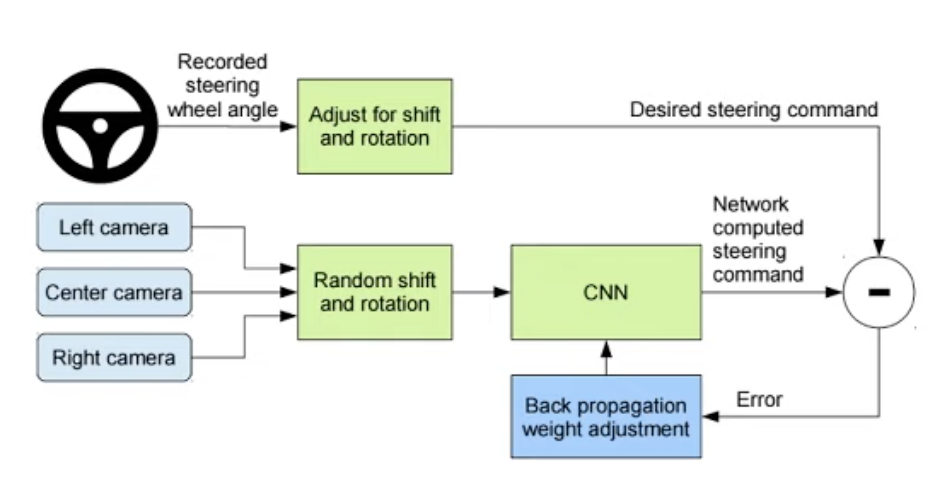
\includegraphics[scale=0.5]{graphics/imitationyes.png}
\end{center}
Essentially, the left and right cameras enabled the vehicle to learn how to correct small errors.  This is a special case of a more general principle, where we learn to train a stable optimal feedback controller, and use this controller to learn a stable policy.  



\subsection{DAgger: Dataset Aggregation}
Another question we could ask is what is the mathematical principle behind the drift?  We are simulating from $\pi_{\theta}(a_t \vert o_t)$, where we sample from $p_{data}(o_t)$, a distribution of training data.  But, when we run the policy, the observation over the policy is different - $p_{\pi_{\theta}}(o_t) \ne p_{data}(o_t)$.  This is a classic distribution shift problem.

\begin{center}
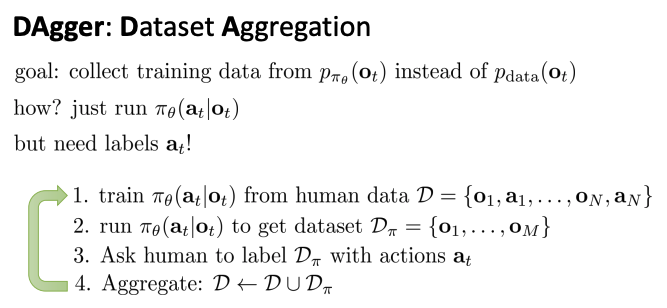
\includegraphics[scale=0.5]{graphics/dagger.png}
\end{center}

The issue with DAgger is that asking a human to label $\mc D_{\pi}$ with actions $a_t$ is not easy, because humans use feedback control - watch the effect of the actions and see the observations.  

\subsection{Deep Imitation In Practice}
Can we make it work without more data? DAgger addresses distributional drift, but what if our model is so good that it doesn't drift?  To do this, we need to mimic expert behavior accurately without overfitting.  

Why might we fail to fit the expert?
\begin{itemize}
\item Even if the observation is fully Markovian, the human behavior might not be Markovian, i. e. depend on additional previous observations.
\item If we have continuous actions, the demonstrator behavior might inconsistently select from multiple modes in the distribution
\end{itemize}

\subsubsection{Non-Markovian Behavior}
To address the Markovian problem, we can use a neural network to encode the images into an RNN state, and use the sequential RNN states to output an action.  We could also use an LSTM cell, which performs better in practice. However, we have the issue of \textbf{causal confusion}.

\begin{center}
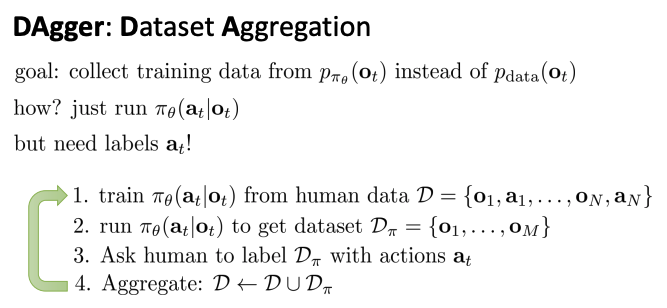
\includegraphics[scale=0.5]{graphics/dagger.png}
\end{center}
Adding a breaklight in the above example makes it difficult to determine whether the breaking is determined by the light or by the pedestrian in the board.  Does DAgger mitigate causal confusion?

\subsubsection{Multimodal Behavior}
When we have multimodal distributions, it is difficult to use the mean and the variance to understand the high probability possibilities: for example, if we want to move left and right with high probability but to the middle with low probability, the mean is the middle option, which should be low probability.

We have a couple of methods for addressing this:
\begin{itemize}
\item Output a mixture of Gaussians. These are sometimes called Mixture Density Networks. The idea is we output $w_1, \mu_1, \Sigma_1, \dots, w_N, \mu_N, \sigma_N$ and output $\pi(a \vert o) = \sum_{i} w_i \mc N(\mu_i, \Sigma_i)$. Some problems with this is that we need more output parameters, and the number of mixture elements we need grows exponentially with the number of dimensions.
\item A more sophisticated option is a Latent variable model.  In this, we output a Gaussian, but we also input a latent variable $\xi \sim \mc N(0, I)$.  We can show in theory that such a model can represent arbitrary distributions.  Some examples are the conditional variational autoencoder, normalizing flows, or Stein variational gradient descent. 
\item If we have discrete options, multimodal distributions are not an issue since the number of bins we need for discretizing a continuous action space grows exponentially with the dimension.   Autoregressive discretization discretizes one dimension at a time. 
\begin{enumerate}
\item First, we discretize the first dimension. Then, we sample from the softmax and obtain a value of the first dimension.
\item Then, we feed the value into another neural network that outputs a distribution over the second dimension.  
\item Repeat the process over all the dimensions.
\end{enumerate}
\end{itemize} 
\subsection{Cost/Reward Functions}
In imitation learning, the humans need to provide data, which is typically finite.  Deep learning methods work well when there is a large amount of data.  Furthermore, humans are not good at providing some kinds of actions.  

We will try to get our machines to learn autonomously, like humans do.  Namely, we try to minimize the objective
$$\min_{\theta} E_{s_{1:T}, a_{1:T}}\left[ \sum_{t} c(s_t, a_t)\right]$$
where $c(s_t, a_t)$ is a cost function.  We could also replace this with the maximization of a reward $r(s_t, a_t)$.

\subsubsection{Cost Function for Imitation}
Some examples are $r(s, a) = \log p(a = \pi^*(s) \vert s)$ or $c(s, a) = 1 - \delta_{a = \pi^*(s)}$.

\end{document} 